\documentclass{beamer}
\usepackage[brazil]{babel}
\usepackage[utf8]{inputenc}
\usepackage[T1]{fontenc}
\usepackage{array}
\usepackage{listings}

%%%%%%%%%%%%%%%%%%%%%%%%%%%%%%%%%%%%%%%%%%%%%%%%%%%%%%%%%%%%%%%%%%%%%%%%%%%%%%%%
%
%  \zoombox[box line width]{contents}
%
%  optimized version for beamer: in full screen, zoom boxes are centred
%  in the viewer; useable with any documenclass
%
%%%%%%%%%%%%%%%%%%%%%%%%%%%%%%%%%%%%%%%%%%%%%%%%%%%%%%%%%%%%%%%%%%%%%%%%%%%%%%%%
\makeatletter
\newsavebox\zb@x
\newcounter{z@@m}
\usepackage{calc}
\newdimen\B@r\newdimen\P@r
\newdimen\@zw\newdimen\@zh\newdimen\@zd

\newcommand{\zoombox}[2][0]{%
  \leavevmode%
  \sbox\zb@x{#2}%
  \setlength\B@r{1pt*\ratio{\wd\zb@x}{\ht\zb@x+\dp\zb@x}}%
  \setlength\P@r{1pt*\ratio{\paperwidth}{\paperheight}}%
  \ifdim\B@r>\P@r\relax%
    \setlength\@zw{\wd\zb@x}\setlength\@zh{\@zw*\ratio{\paperheight}{\paperwidth}}%
    \setlength\@zd{(\@zh-\ht\zb@x-\dp\zb@x)*\real{0.5}+\dp\zb@x}%
    \setlength\@zh{\@zh-\@zd}%
  \else%
    \setlength\@zh{\ht\zb@x+\dp\zb@x}%
    \setlength\@zw{\@zh*\ratio{\paperwidth}{\paperheight}}%
    \setlength\@zh{\ht\zb@x}\setlength\@zd{\dp\zb@x}%
  \fi%
  \makebox[0pt][l]{\makebox[\wd\zb@x][c]{\makebox[\@zw][l]{%
    \pdfdest name {zbfs\thez@@m} fitr
      width  \@zw\space
      height \@zh\space
      depth  \@zd\space
  }}}%
  \pdfdest name {zb\thez@@m} fitr
    width  \wd\zb@x\space
    height \ht\zb@x\space
    depth  \dp\zb@x\space
  \immediate\pdfannot 
    width  \wd\zb@x\space
    height \ht\zb@x\space
    depth  \dp\zb@x\space
  {%
    /Subtype/Link/H/N
    /Border [0 0 #1 [1 2]]
    /A <<
      /S/JavaScript
      /JS (
        if(typeof(zoomed)=='undefined'||!zoomed){
          var lastView=this.viewState;
          if(app.fs.isFullScreen) this.gotoNamedDest('zbfs\thez@@m');
          else this.gotoNamedDest('zb\thez@@m');
          zoomed=true;
        }else{
          this.viewState=lastView;
          zoomed=false;
        }
      )
    >>
  }%
  \usebox{\zb@x}%
  \stepcounter{z@@m}%
} 
\makeatother
%%%%%%%%%%%%%%%%%%%%%%%%%%%%%%%%%%%%%%%%%%%%%%%%%%%%%%%%%%%%%%%%%%%%%%%%%%%%%%%


\usetheme{Laughlin}

\begin{document}
\title{Seminário de Andamento de Doutorado - Extração de Dados Estruturados}
%\author[Roberto Panerai Velloso]{Orientando: Roberto Panerai Velloso \\
%Orientadora: Carina F. Dorneles \\ \{rvelloso, dorneles\}@gmail.com }
\author[Roberto Panerai Velloso]{Roberto Panerai Velloso, Carina F. Dorneles \\ 
\{rvelloso, dorneles\}@gmail.com}
%\date{\today}
\date{}
%\institute{Universidade Federal de Santa Catarina}
\institute{
%UFSC - Universidade Federal de Santa Catarina \\ PPGCC - Programa de
% Pós-Graduação em Ciência da Computação
\begin{figure}[H]
  \label{fig:logo1}
    
\includegraphics[scale=0.50]{img/brasao_ufsc_80.png}
    
\includegraphics[scale=0.30]{img/brasao_418.png}
\end{figure}
%\begin{figure}[H]
%  \label{fig:logo2}
%    
\includegraphics[scale=0.30]{brasao_ufsc_80.png}
%\end{figure}
}

\frame{
\titlepage
} 

\frame{\frametitle{Sumário}
\begin{small}
\tableofcontents
\end{small}
}

\section{Introdução}
%\frame{\tableofcontents[currentsection]}

\subsection{Contexto}
\frame{\frametitle{Contexto}
\begin{itemize}
\item Obter informação estruturada (\textit{i.e.}, relacional) a partir de
fontes não estruturadas ou semiestruturadas.

\item Dados são disponibilizados na \textit{web} para serem consumidos por
pessoas, não por máquinas.

\item Motivação
\begin{itemize}
  \item realizar consultas com SQL;
  \item criar bases de dados para domínios específicos;
  \item enriquecer outras aplicações;
  \item criar taxonomias.
\end{itemize}
\end{itemize}
}

\subsection{Problema}
\frame{\frametitle{Extração de Dados Estruturados}
\begin{itemize} 
	\item Extração a partir de fontes semiestruturadas;
	\item Utilização de informação sintática;
	\item Requisitos de escalabilidade:
	\begin{itemize}
	  \item nível de supervisão;
	  \item generalidade;
	  \item precisão vs \textit{recall}. 
\end{itemize}
\end{itemize}
}

\subsection{Objetivo}
\frame{\frametitle{Objetivo Geral} 
O objetivo geral desta pesquisa é desenvolver um método automático (não
supervisionado) de extração de dados estruturados a partir de informação
semiestruturada contida em páginas \textit{web}.
}

\frame{\frametitle{Objetivos específicos}
\begin{itemize}
\item desenvolver um método de \textbf{segmentação} de um documento HTML que
identifique as regiões da página com conteúdo semiestruturado;
\item desenvolver um método de \textbf{filtragem} que identifique quais das
regiões semiestruturadas possuem conteúdo e quais possuem ruído (menus, \textit{template}, anúncios,
etc.);
\item desenvolver um método de estruturação da informação semiestruturada
identificada (\textit{e.g.} \textbf{alinhamento} de registros);
\item desenvolver um \textbf{\textit{framework}} de extração estruturada;
\item criar \textbf{\textit{datasets}} com ampla cobertura para avaliação de
métodos de extração;
\end{itemize}
}

\subsection{Contribuições}
\frame{\frametitle{Contribuições}
\begin{itemize}
  \item desenvolvimento de um novo método de extração estruturada;
  \item criação de \textit{datasets} com ampla cobertura para avaliação de
  métodos de extração estruturada;
  \item proposição de novas métricas;
  \item publicação dos resultados da pesquisa em eventos e periódicos;
  \item desenvolvimento de um \textit{framework} de extração estruturada. 
\end{itemize}
}

\section{Trabalhos Relacionados} 
\frame{\frametitle{Trabalhos Relacionados}
\begin{itemize}
\item Poucas implementações disponíveis;
\item Alguns datasets disponíveis; 
\item Três principais abordagens identificadas:
\begin{itemize}
  \item extração de tabelas e listas;
  \item extração a partir de uma única página;
  \item extração a partir de múltiplas páginas.
\end{itemize}
\end{itemize}
}

\subsection{Tabelas e Listas}
\frame{\frametitle{Extração de Tabelas e Listas}
Abordagens fazem suposições \textbf{fortes} a respeito da entrada.
\begin{itemize}
  \item WebTables Google/ACSDb (\texttt{<table>}) (2008);
  \item WebTables M\$/Probase (\texttt{<table>}) (2012);
  \item ListExtract (\texttt{<ol/ul/etc.>}) (2009);
  \item Tegra (ListExtract da M\$) (\texttt{<ol/ul/etc.>}) (2015);
  \item \textit{Top-k pages} (\textit{template} fixo) (2013).
\end{itemize}
}

\subsection{Única Página}
\frame{\frametitle{Extração a partir de uma única página}
Buscam padrões no HTML/DOM para encontrar os registros. Ao menos dois registros
devem existir para ser possível a extração.
Algumas abordagens ``gerais'':
\begin{itemize}
  \item Abordagens não visuais: MDR, NET, TPC (2003 - 2009);
  \item Abordagens visuais: DEPTA, ViPER, ClustVX, AutoRM, (CHU et al., 2015b)
  (2005 - 2015);
\end{itemize}
}

\subsection{Múltiplas Páginas}
\frame{\frametitle{Extração a partir de múltiplas páginas}
Utilizam uma ``amostra'' do \textit{template} do \textit{site} para treinamento.
São capazes de extrair conteúdo de páginas com apenas um registro.
(\textit{i.e.}, páginas de detalhe).
\begin{itemize}
  \item RoadRunner (2001);
  \item ExAlg (2003);
  \item FiVaTech (2010).
\end{itemize} 
}

\section{Proposta}

\subsection{Características}
\frame{\frametitle{Características}
\begin{itemize}
  \item Independente de domínio;
  \item Independente de características da linguagem HTML; 
  \item Não dependa de bases de dados e/ou definições \textit{a priori}.
  \item Totalmente automática;
  \item Necessite de apenas uma página (ao invés de um conjunto de páginas);
  \item Não dependa de treinamento;
  \item Computacionalmente eficiente.
\end{itemize}
}

\subsection{Suposições}
\frame{\frametitle{Suposições}
\begin{enumerate}
\item \textbf{Segmentação}: diferentes
regiões de uma página HTML são formatadas de maneiras diferentes, justamente
para que haja distinção entre elas, portanto serão formadas por conjuntos de \textit{tag
paths} diferentes, caso contrário não haveria diferença visual
significativa entre as regiões de uma página;
\item \textbf{Registros}: regiões com conteúdo semiestruturado são compostas por
conjuntos de registros contíguos e com estrutura semelhantes, 
descritos por sequências de \textit{tag paths} semelhantes sendo, portanto, regiões cíclicas.
\end{enumerate} 
}

\subsection{Tag Paths}
\frame{\frametitle{$Tag$ $paths$}
\begin{figure}[H]
  \caption{Construção da sequência de $tag$ $paths$ (TPS) a partir do HTML.}
  \centering
    \zoombox{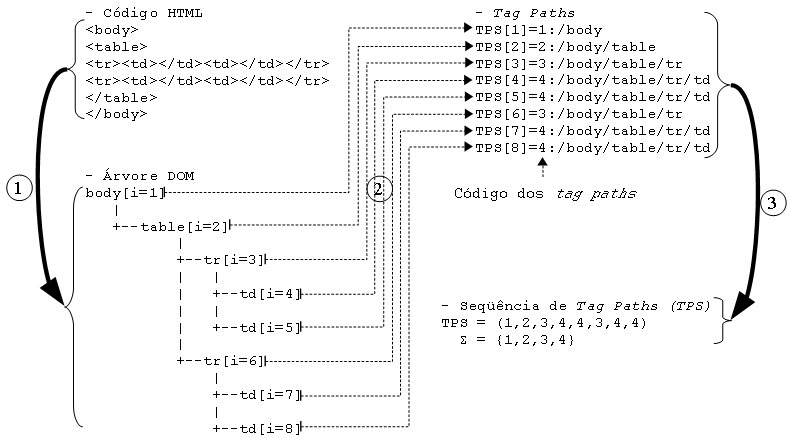
\includegraphics[scale=0.45]{img/example1-pt.jpg}}
\end{figure}
}
\frame{\frametitle{$Tag$ $paths$}
\begin{figure}[H]
  \caption{Construção da sequência de $tag$ $paths$ (TPS) a partir do HTML.}
  \centering
    \zoombox{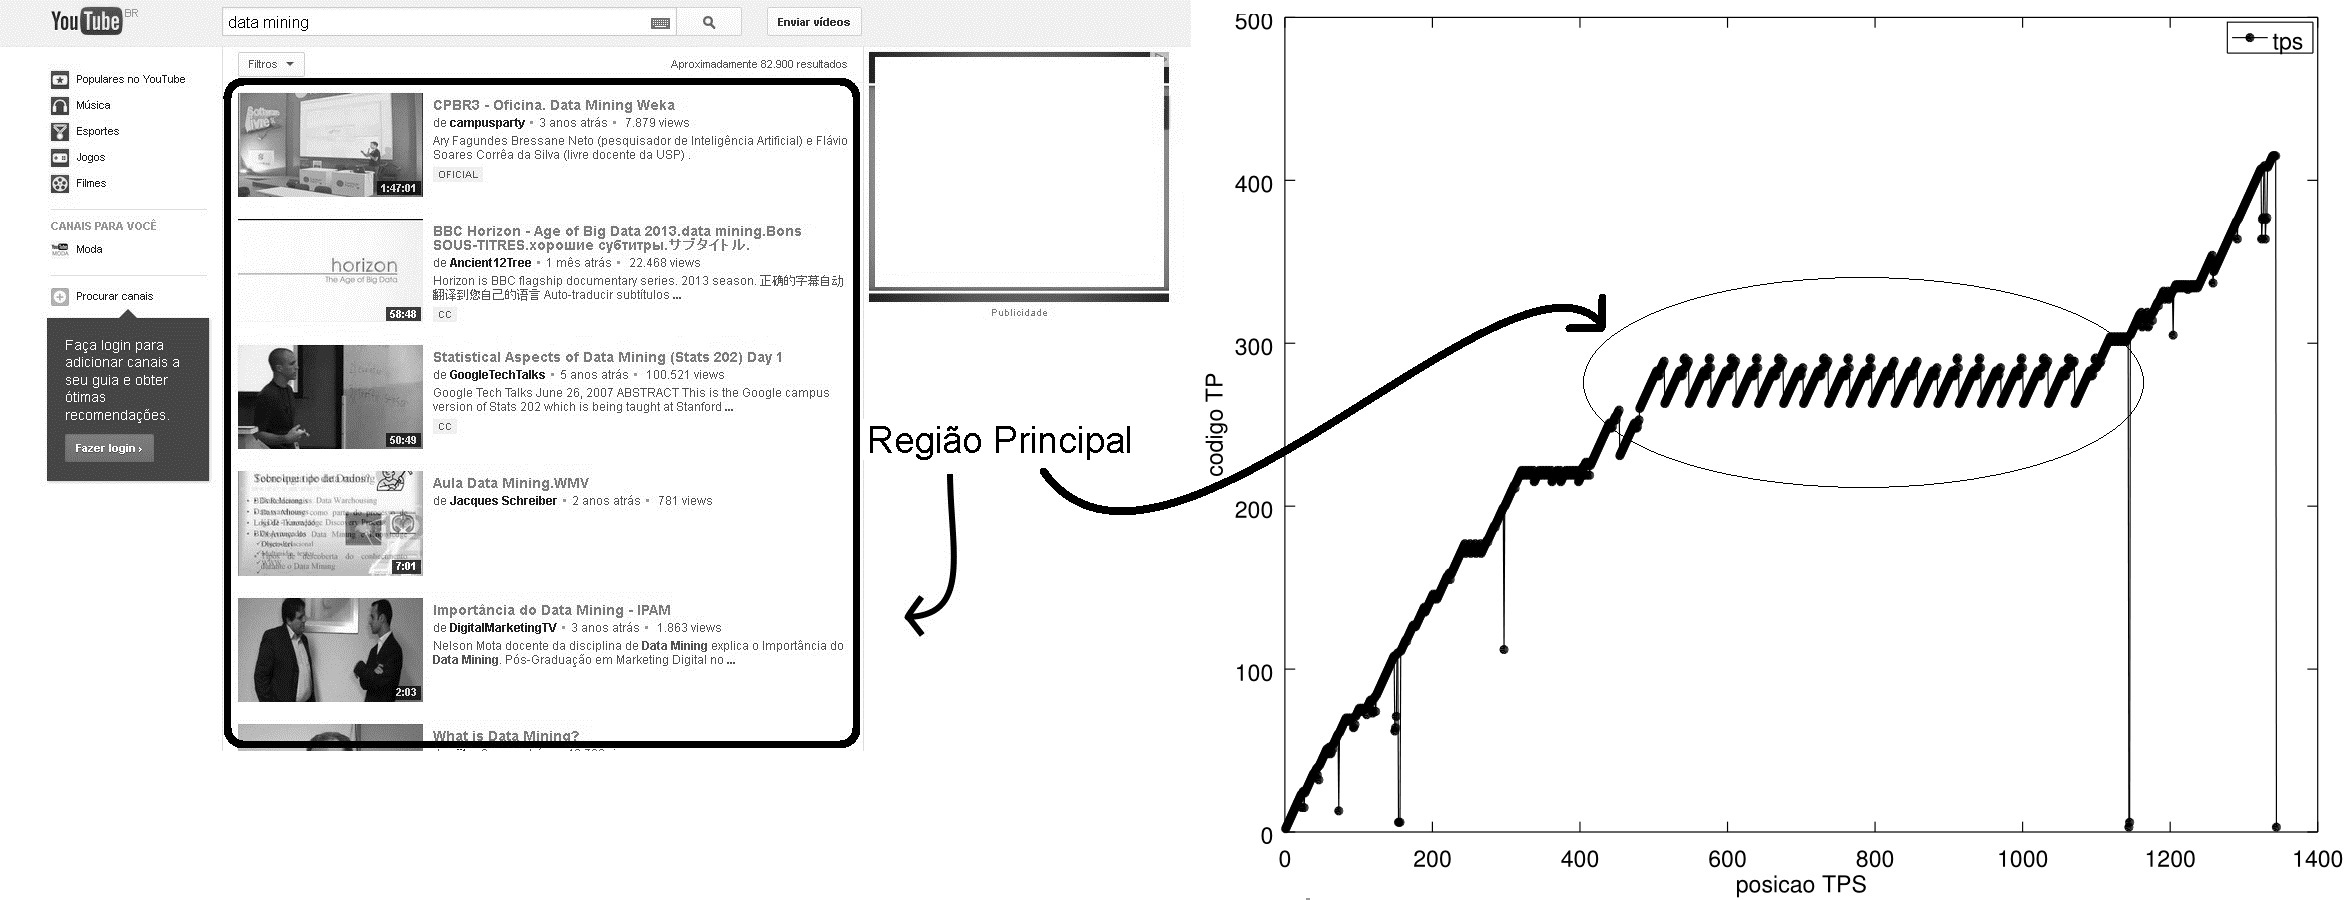
\includegraphics[width=\textwidth]{img/creat-tps-pt.jpg}}
\end{figure}
}

\frame{\frametitle{$Tag$ $paths$}
\begin{figure}[H]
  \caption{Sequência de $tag$ $paths$ (TPS).}
  \centering
    \zoombox{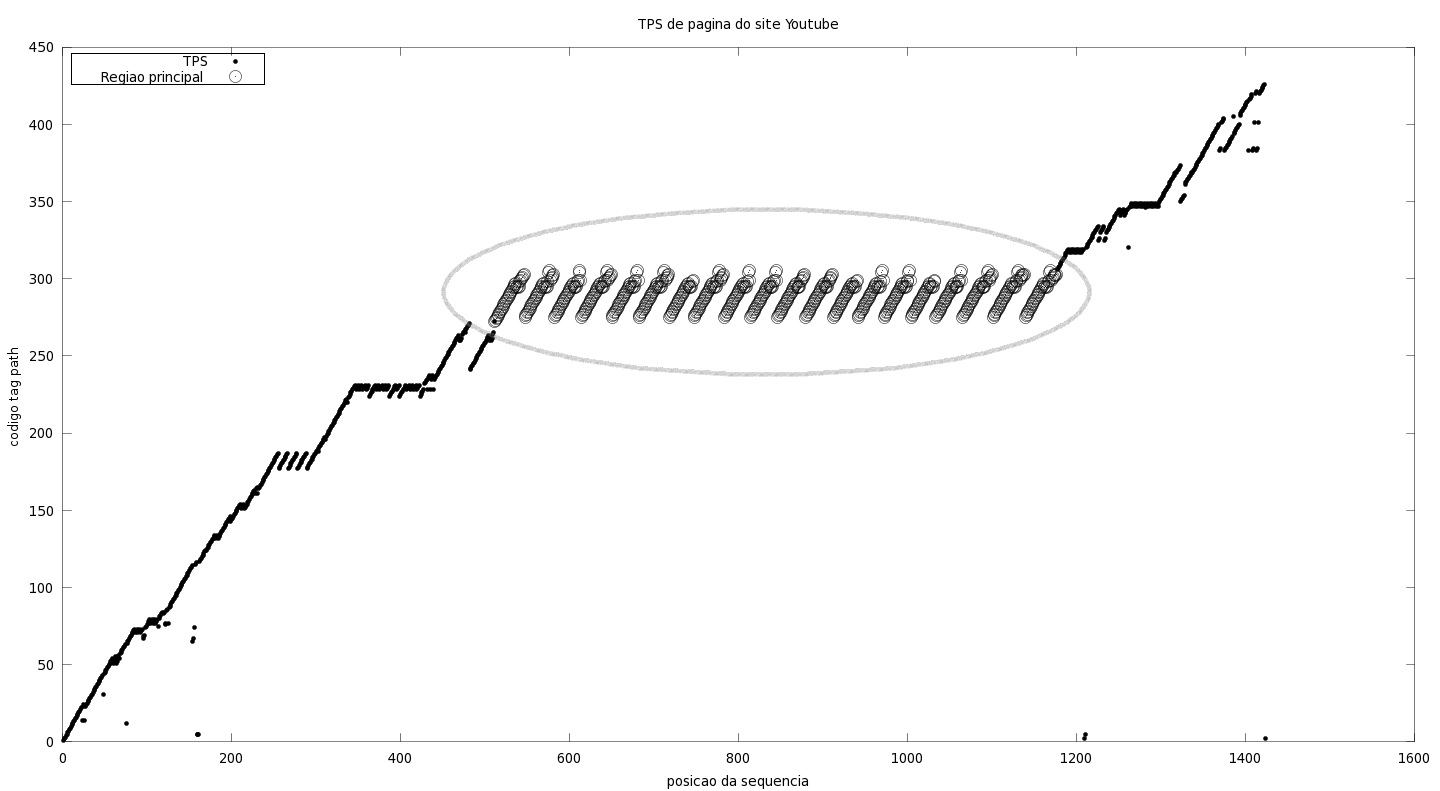
\includegraphics[width=\textwidth]{img/tps-pt.jpg}}
\end{figure}
}

\subsection{Detecção das Regiões Semiestruturadas}
\frame{\frametitle{Contorno superior}
\begin{figure}[H]
  \caption{Contorno superior da TPS.}
  \centering
    \zoombox{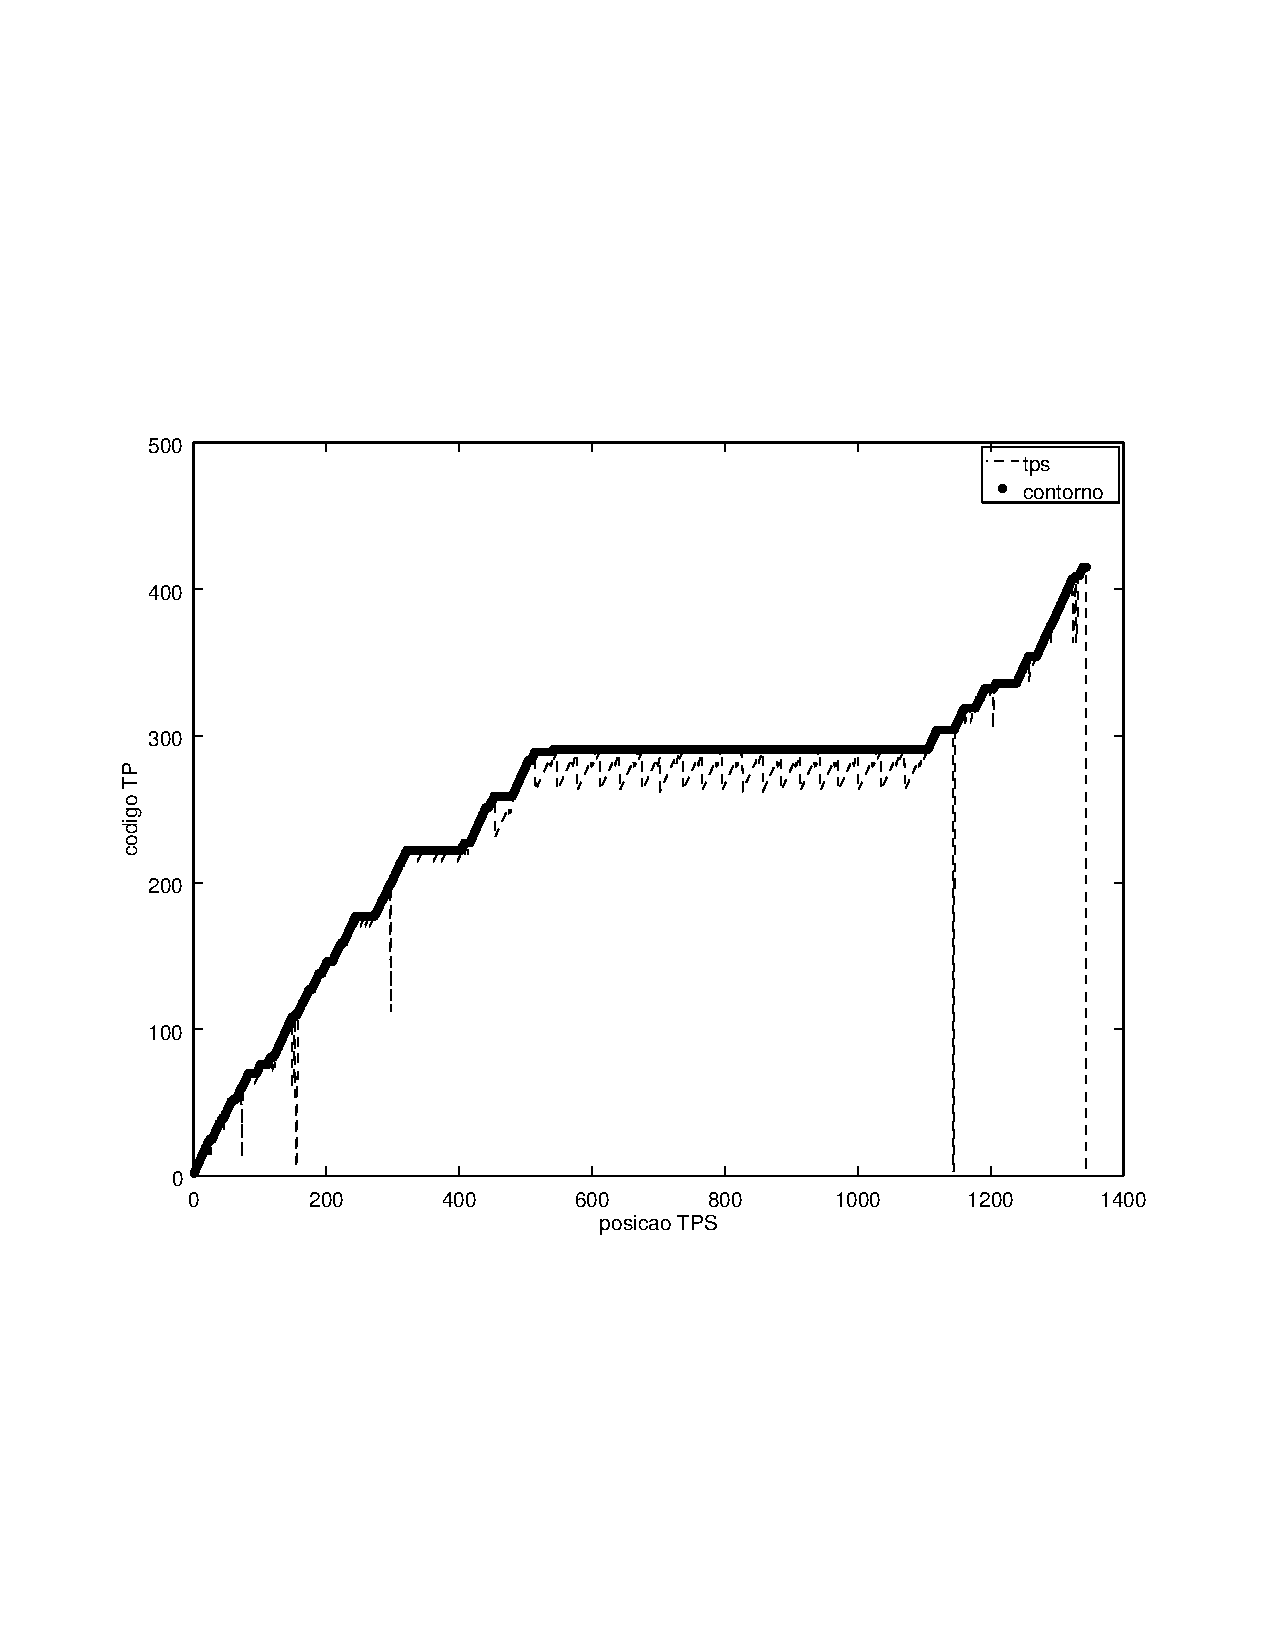
\includegraphics[trim={55 200 40
     210},clip,scale=0.45]{img/contour-pt.pdf}}
\end{figure}
}
\frame{\frametitle{Derivada do Contorno}
\begin{figure}[H]
  \caption{Derivada do contorno superior da TPS.}
  \centering
    \zoombox{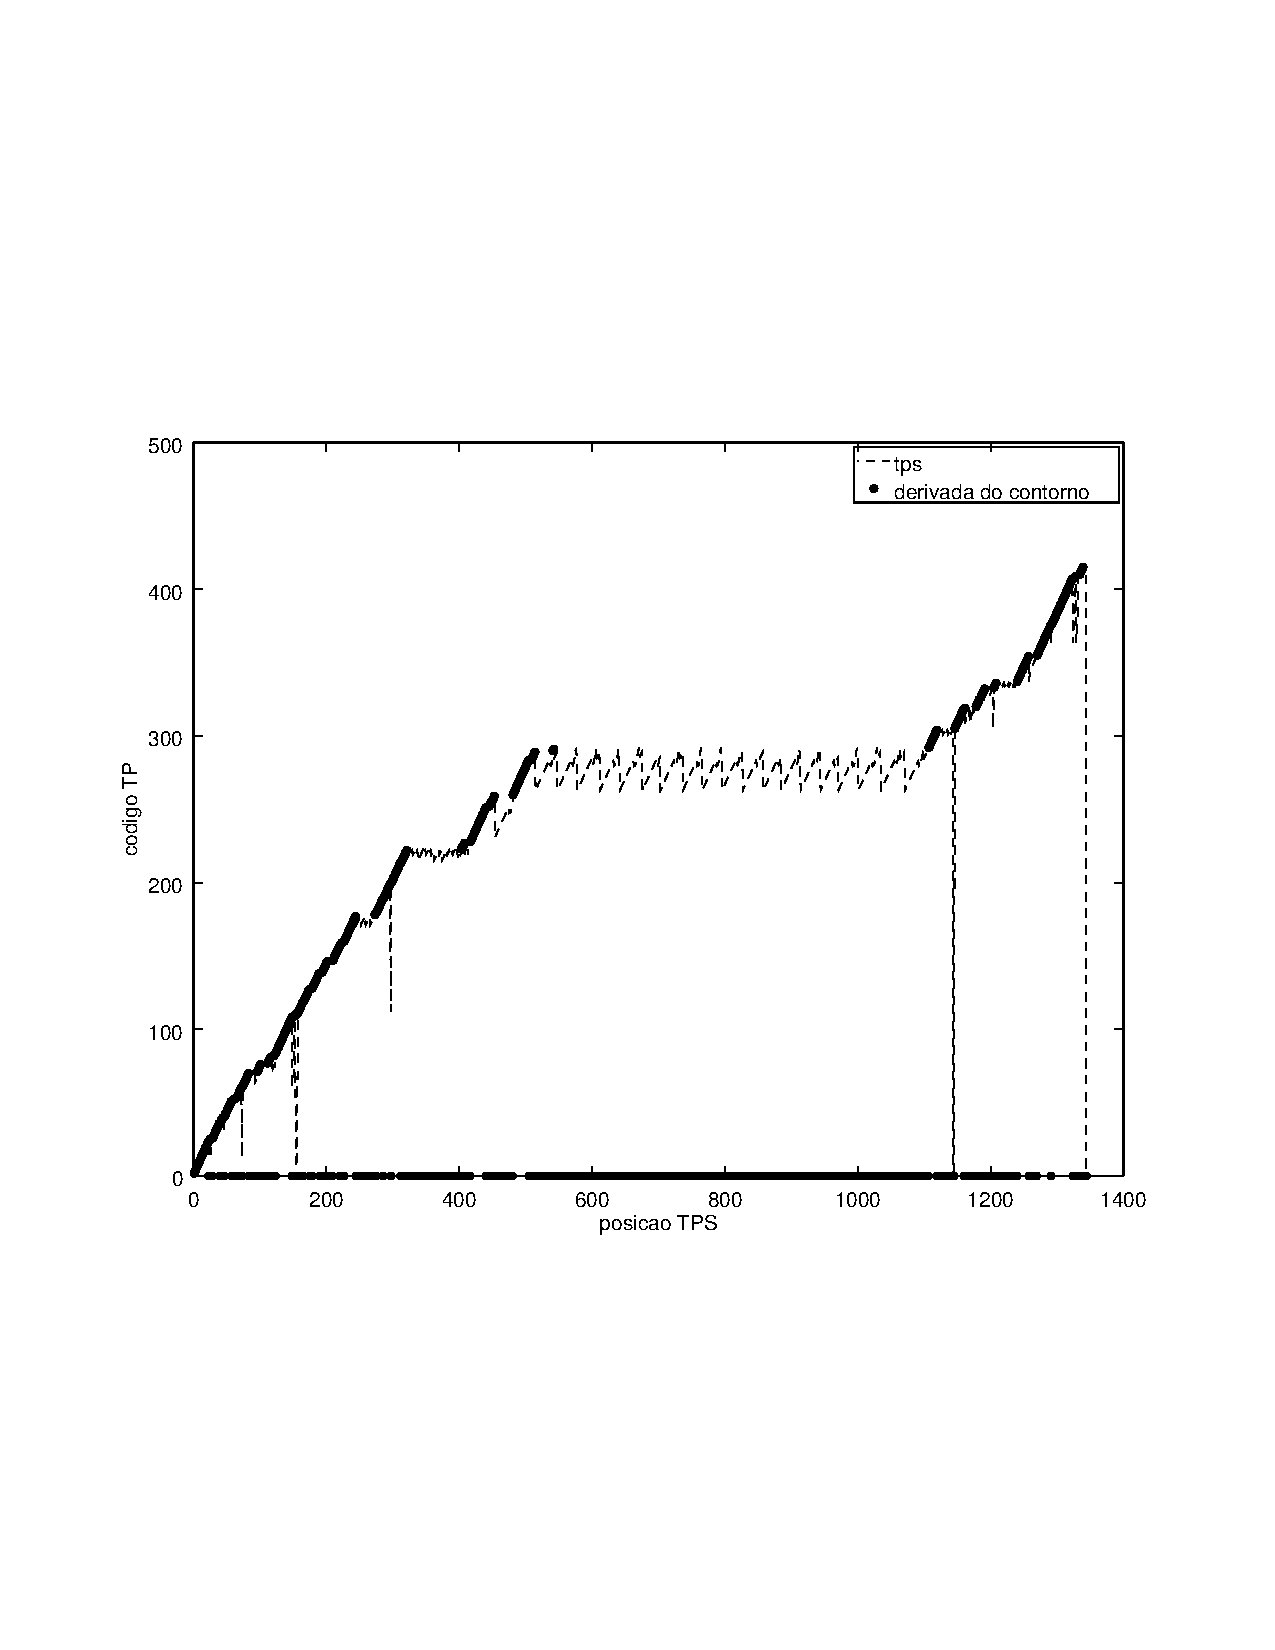
\includegraphics[trim={55 200 40
     210},clip,scale=0.45]{img/derivada-pt.pdf}}
\end{figure}
}
\subsection{Filtragem das Regiões}
\frame{\frametitle{Regressão Linear - Identificação da Estrutura}
\begin{figure}[H]
  \caption{Regressão linear da região.}
  \centering
    \zoombox{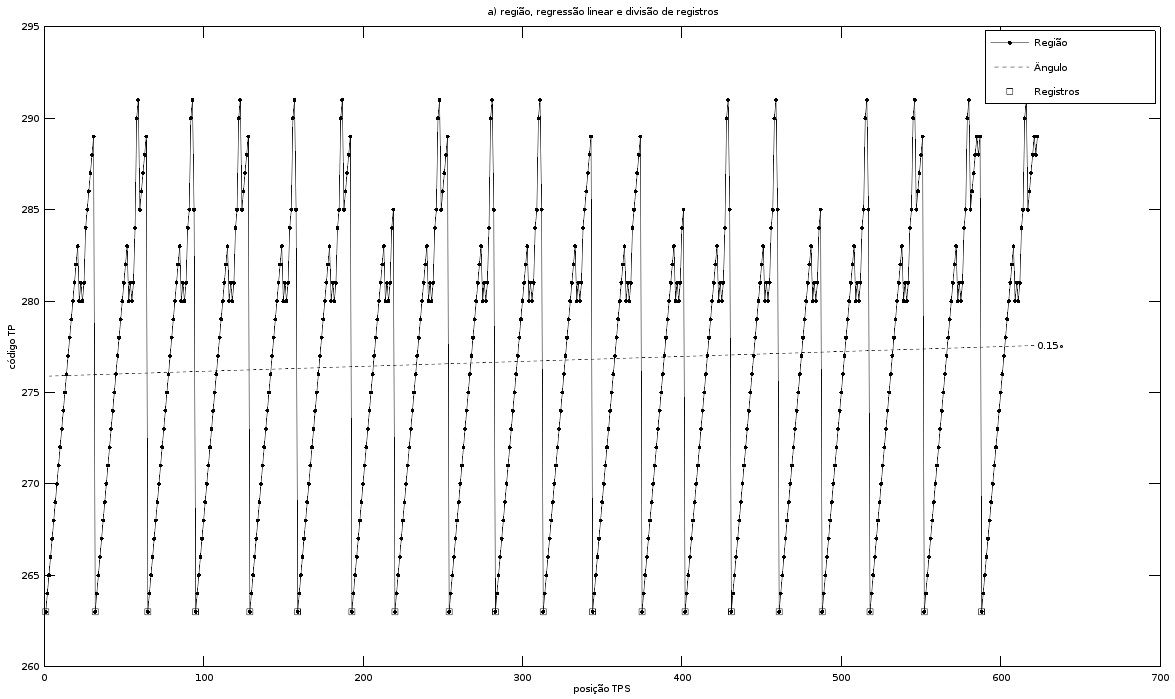
\includegraphics[scale=0.25]{img/region-pt.jpg}}
\end{figure}
}

\frame{\frametitle{Clustering das Regiões - Identificação do Ruído}
\begin{itemize}
\item O \textit{score} da região utilizado para clusterização é diretamente
proporcional ao tamanho da subsequência e inversamente proporcional à distância
que se encontra do centro da sequência completa;
\item É utilizado ``kmeans ótimo de uma dimensão'', forçando a criação de dois
\textit{clusters};
\item O \textit{cluster} com maior centro é considerado conteúdo e o outro
\textit{cluster} (com menor centro) é descartado.
\end{itemize}
}

\subsection{Subdivisão em Registros}
\frame{\frametitle{Estimando tamanho e quantidade de registros}
\begin{figure}[H]
  \caption{a) TPS e regressão linear da região; b) autocorrelação; c) Espectro
  de potência e estimativas de quantidade e tamanho dos registros.}
  \centering
    \zoombox{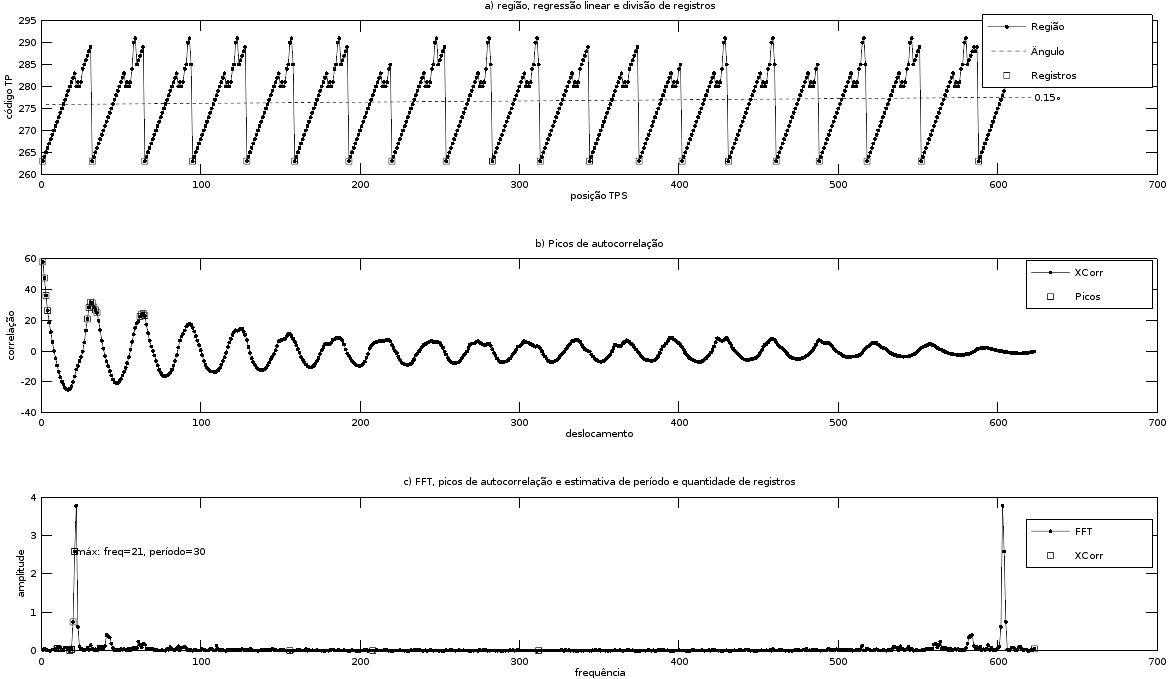
\includegraphics[scale=0.25]{img/fftxcorr-pt.jpg}}
\end{figure}
}

\frame{\frametitle{Identificação dos Registros}
\begin{small}
\begin{equation}\label{eq:scoreSize}
score_{tamanho} = \frac{min(tamanhoMedio, periodoEstimado)}{max(tamanhoMedio,
periodoEstimado)}
\end{equation}
\begin{equation}\label{eq:scoreCount}
score_{quantidade} = \frac{min(quantidade, frequenciaEstimada)}{max(quantidade,
frequenciaEstimada)}
\end{equation}
\begin{equation}\label{eq:scoreCoverage}
score_{cobertura}=\frac{posicaoRegistro_n - posicaoRegistro_1}{tamanhoTotalRegiao}
\end{equation}
\begin{equation}\label{eq:scoreTotal}
score_{total}=\frac{score_{tamanho}+score_{quantidade}+score_{cobertura}}{3}
\end{equation}
\end{small}
}

\subsection{Alinhamento dos Registros}
\frame{\frametitle{Center Star}
Como o alinhamento ótimo de múltiplas sequências é \textit{NP-Hard},
alternativas aproximadas, com complexidade polinomial, devem ser empregadas.

\begin{itemize}
\item Características do algoritmo \textit{Center Star}:
\begin{itemize}
  \item Não encontra necessariamente a solução ótima;
  \item Tem complexidade computacional polinomial $O(N^2\cdot n)$;
  \item Garante um erro máximo com relação à solução ótima.
\end{itemize}
\end{itemize}
}

\section{Cronograma}
\frame{\frametitle{Cronograma da pesquisa}
\begin{enumerate}
  \item \textbf{levantamento bibliográfico}: leitura de publicações para
  levantamento do estado da arte \textbf{(até 12/2018)};
  \item \textbf{realização de experimentos}: realização de testes e experimentos com a
  abordagem proposta utilizando \textit{datasets} disponíveis publicamente
  para comparação com as demais abordagens existentes \textbf{(até 12/2016)};
  \item \textbf{publicação dos artigos}: escrita e publicação de artigos em
  congressos e periódicos \textbf{(até 12/2017)};
  \item \textbf{disponibilização do \textit{framework}}: finalização da codificação do
  \textit{framework} C++/Lua, documentação da API e disponibilização pública
  \textbf{(até 12/2017)};
  \item \textbf{qualificação}: exame de qualificação \textbf{(até 6/2017)};
  \item \textbf{defesa}: escrita da tese e defesa final \textbf{(até 12/2018)}.
\end{enumerate}
}
\end{document}
